\documentclass[a4paper,14pt]{extreport}

\usepackage[T1,T2A]{fontenc}
\usepackage[utf8]{inputenc}
\usepackage[figure,table]{totalcount}
\usepackage{subcaption}
\usepackage{graphicx}
\graphicspath{ {images/} }
\usepackage{mathtools}

\usepackage{../packages/bsumain}
\usepackage{../packages/titlepage}
\usepackage{blindtext}
\newcommand{\quotes}[1]{``#1"}

\jobtitle{Матричные игры. Сетевые задачи}
\labnum{2}

\begin{document}
\maketitle
\setcounter{page}{2}

\chapter{Графоаналитический метод решения матричных игр}
Найти графоаналитическим методом решение матричной игры з матрицей $H$\par

\section{Задача 10b (ч1 стр. 29)}
\subsection{Условие}
\begin{equation}
    H = \begin{pmatrix} 
            -2 & 4 & 1 & 3 & -2 \\ 
            1 & 5 & 2 & 3 & 7 \\
            -1 & 3 & 3 & 3 & 1 \\
            2 & 0 & -2 & -2 & 2
        \end{pmatrix}
\end{equation}

\subsection{Решение}
Найдём верхнее и нижнее значения игры:
\begin{equation*}
    \alpha_1 = -2, 
    \alpha_2 = 1,
    \alpha_3 = -1,
    \alpha_4 = -2
\end{equation*}
\begin{equation*}
    \beta_1 = 2,
    \beta_2 = 5,
    \beta_3 = 3,
    \beta_4 = 3,
    \beta_5 = 7
\end{equation*}

$ \alpha = 1 \neq \beta = 2 $ - чистых стратегий нет!\\

Будем исключать доминирующие стратегии: \par
Пусть стратегии первого игрока $A_i, i=\overline{1, 4}$ - , а второго - $B_j, j=\overline{1, 5}$ \par
Доминирование будем обозначать, как \quotes{\gg}

\begin{equation*}
     ([1, 5, 2, 3, 7] \geq [-2, 4, 1, 3, -2]) \implies A_2 \gg A_1 \implies p_1 = 0
\end{equation*}
\begin{equation*}
    ([-2, 1, -1, 2] \leq [-2, 7, 1, 2]) \implies B_1 \gg B_5 \implies q_5 = 0
\end{equation*}
\begin{equation*}
    ([1, 2, 3, -2] \leq [4, 5, 3, 0]) \implies B_3 \gg B_2 \implies q_2 = 0
\end{equation*}
\begin{equation*}
    ([1, 2, 3, -2] \leq [3, 3, 3, -2]) \implies B_3 \gg B_4 \implies q_4 = 0
\end{equation*}

Имеем:
\begin{equation}
    H = \begin{pmatrix}
        1 & 2 \\
        -1 & 3 \\
        2 & -2
        \end{pmatrix}
\end{equation}

Построим график: \newpage

\begin{figure}[ht]
    \centering
    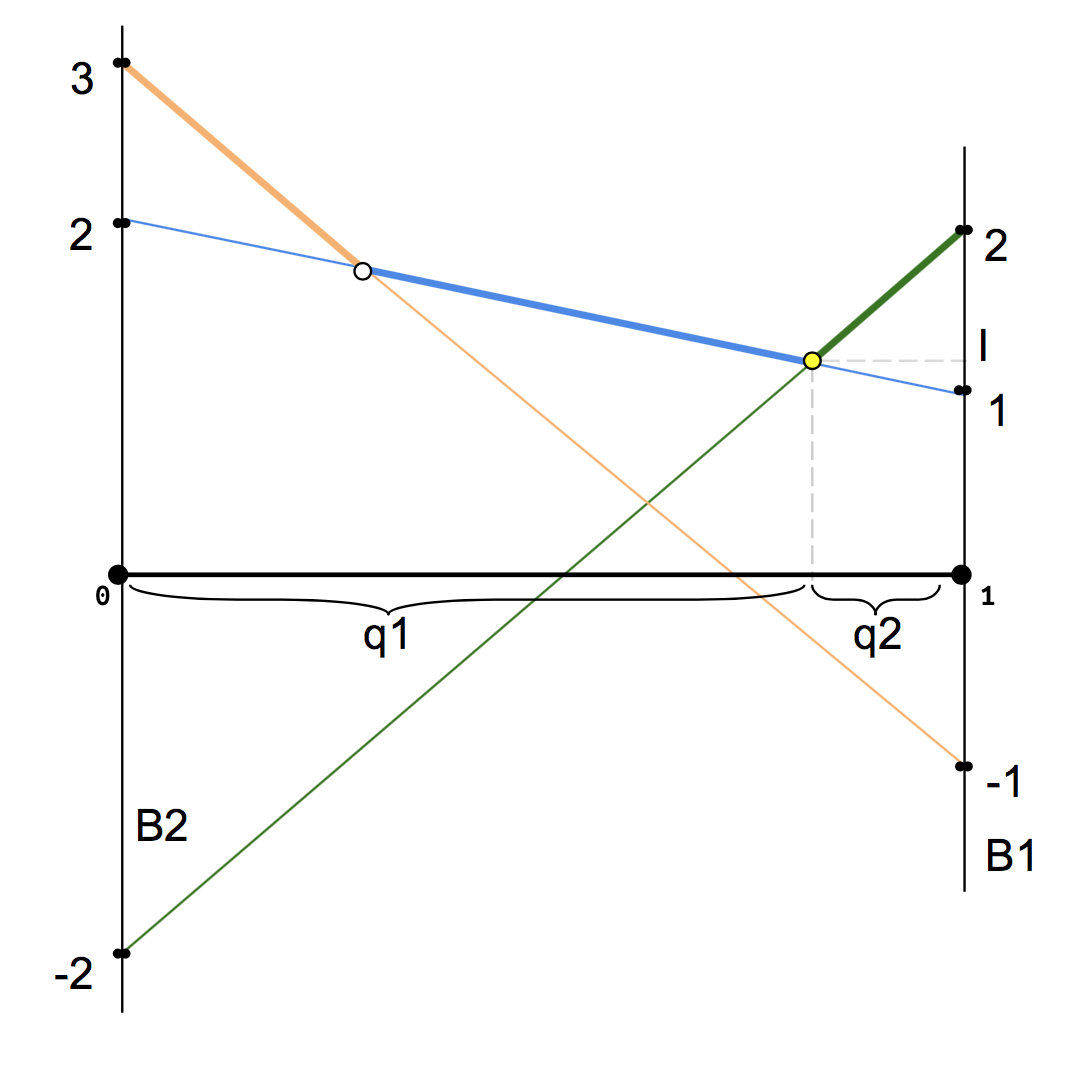
\includegraphics[width=0.6\textwidth]{plot.png}
    \caption{Оптимальная точка - пересечение синей и зелёной стратегий}
\end{figure}

Запишем систему уравнений для оптимальной точки:
\begin{equation}
\begin{cases}
    1 + q_2 = I \\
    2 - 4q_2 + I
\end{cases}
\end{equation}

Откуда: $q_2 = \frac{1}{5}, I=\frac{6}{5} \implies q_1 = \frac{4}{5}$\\

Исключив стратегию $A_2$ (зеленую) как проигрышную, \par
запишем систему для стратегий $A_1$, $A_3$ первого игрока:
\begin{equation}
\begin{cases}
    p_1 + 2p_3 = I \\
    2p_1 - 2p_3 = I \\
    p_1 + p_3 = 1
\end{cases}
\end{equation}

Откуда: $p_1 = \frac{4}{5}, p_3 = \frac{1}{5}$\\

Переходя к исходной размерности запишем ответ:
\begin{equation*}
\begin{multlined}
    I = \frac{6}{5}\\
    p = (0, \frac{4}{5}, 0, \frac{1}{5})\\
    q = (\frac{4}{5}, 0, \frac{1}{5}, 0, 0)
\end{multlined}
\end{equation*}


\section{Задача 2d (ч1 стр. 21)}
\subsection{Условие}
\begin{equation}
    H = \begin{pmatrix} 
            2 & 4 & 1 & 5 & 1 \\ 
            5 & 2 & 3 & 0 & -1 \\
            2 & -2 & 4 & -3 & 0
        \end{pmatrix}
\end{equation}

\subsection{Решение}
Найдём верхние и нижние значения игры
\begin{equation*}
\begin{multlined}
    \alpha = 1, i_0 = 1\\
    \beta = 1, j_0 = 5
\end{multlined}
\end{equation*}

Следовательно: $I=1$, $A_1$ и $B_5$ - оптимальные чистые стратегии первого\par и второго игроков соответственно. \\

Докажем это с помощью графического метода:\par
Сведём задачу к меньшей размерности, исключив любые строки/столбцы\par
кроме $A_1$ и $B_5$ - так как они доминирующие, имеем:

\begin{equation*}
    q_1 = 0, q_3 = 0, p_2 = 0
\end{equation*}

\begin{equation}
    H = \begin{pmatrix} 
            4 & 5 & 1 \\ 
            -2 & -3 & 0
        \end{pmatrix}
\end{equation}

Построим график:
\begin{figure}[h]
    \centering
    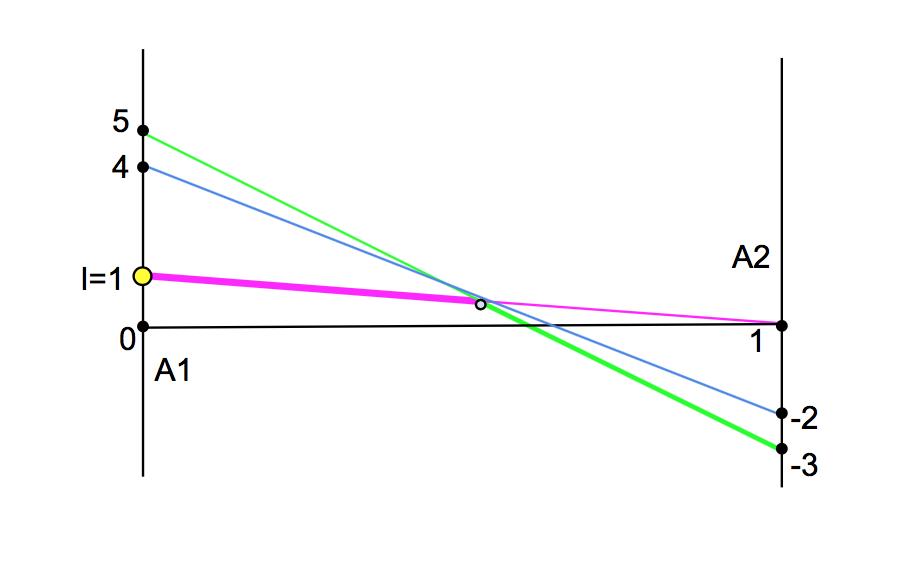
\includegraphics[width=0.7\textwidth]{plot2.png}
    \caption{Оптимальная точка соответствует чистой стратегии}
\end{figure}

Ответ: $I = 1,p = (1, 0, 0),q = (0, 0, 0, 0, 1)$

\chapter{Сетевые задачи}
\section{Задача 1b (ч2 стр. 8)}
\subsection{Условие}
Для приведенных ниже неориентированных связных графов найти\par минимальное и максимальное остовные деревья
\begin{figure}[h]
    \centering
    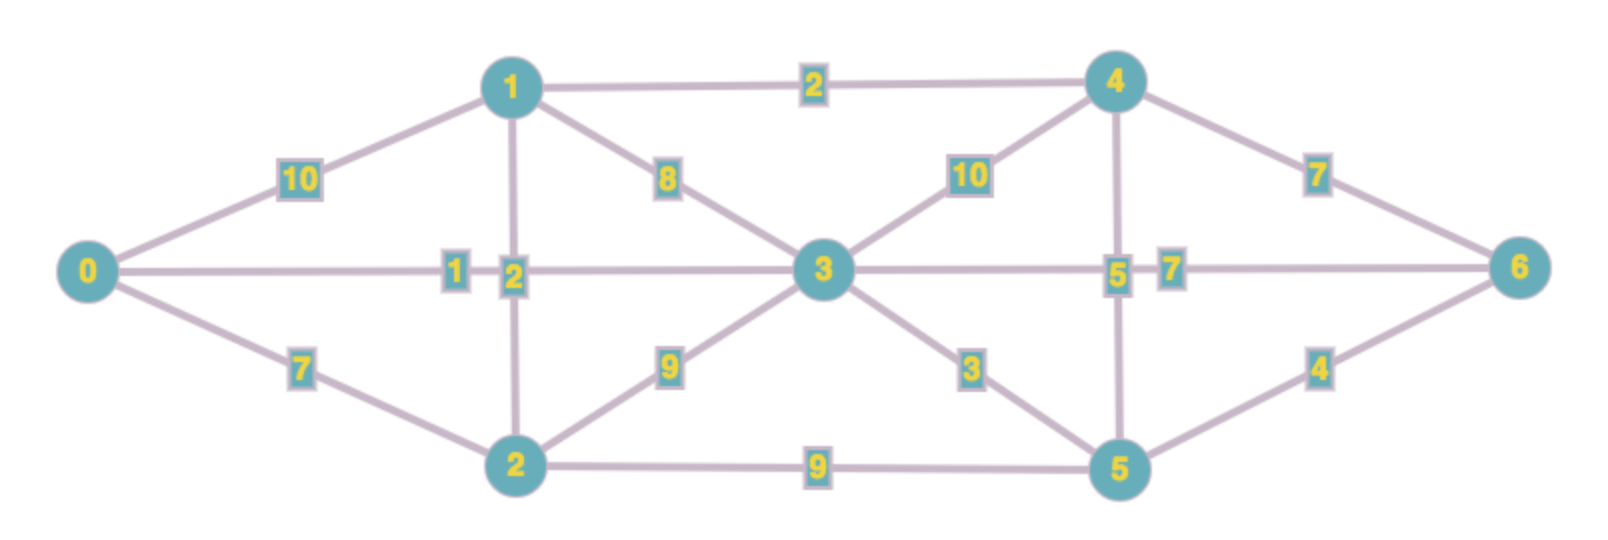
\includegraphics[width=0.8\textwidth]{graph.png}
\end{figure}
\subsection{Решение}
Будем использовать алгоритм Крускала:\par
Упорядочим рёбра по неубыванию весов
\begin{equation*}
\begin{multlined}
    (0,3) \to 1\\
    (1,2) \to 2\\
    (1,4) \to 2\\
    (3,5) \to 3\\
    (5,6) \to 4\\
    (4,5) \to 5\\
    (0,2) \to 7\\
    (3,6) \to 7\\
    (4,6) \to 7\\
    (1,3) \to 8\\
    (2,3) \to 9\\
    (2,5) \to 9\\
    (0,1) \to 10\\
    (3,4) \to 10\\
\end{multlined}
\end{equation*}\\

Добавляем рёбра в остов:\par
\begin{equation*}
    (0,3) \to (1,2) \to (1,4) \to (3,5) \to (5,6) \to (4,5): [|I| = n-1] \implies stop
\end{equation*}

\begin{figure}[h]
    \centering
    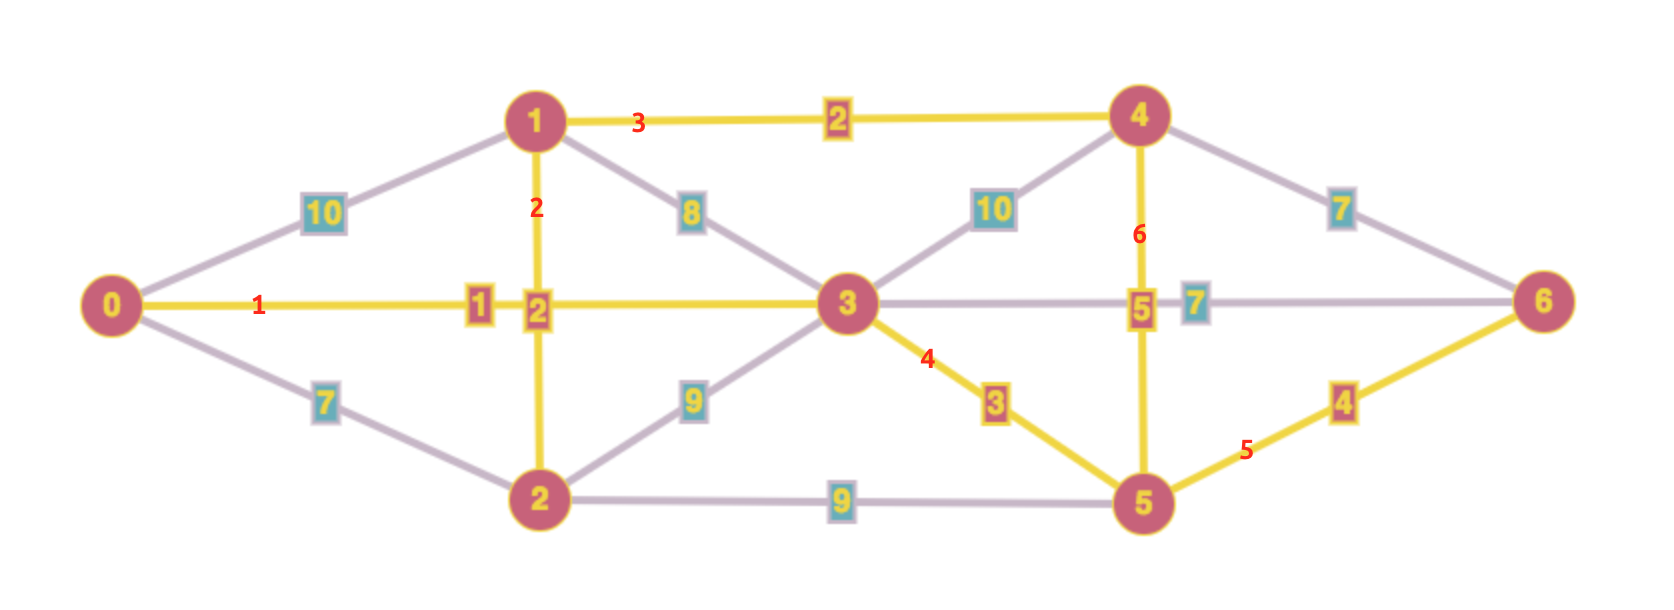
\includegraphics[width=0.8\textwidth]{graph2.png}
    \caption{Минимальный остов минимального веса}
\end{figure}

Вес остова: $W_{min} = 1+2+2+3+4+5=17$ \\

Для минимального остовного дерева максимального веса аналогично:
\begin{equation*}
    (3,4) \to (0,1) \to (2,5) \to (2,3) \to (1,3) \to (4,6): [|I| = n-1] \implies stop
\end{equation*}

\begin{figure}[h]
    \centering
    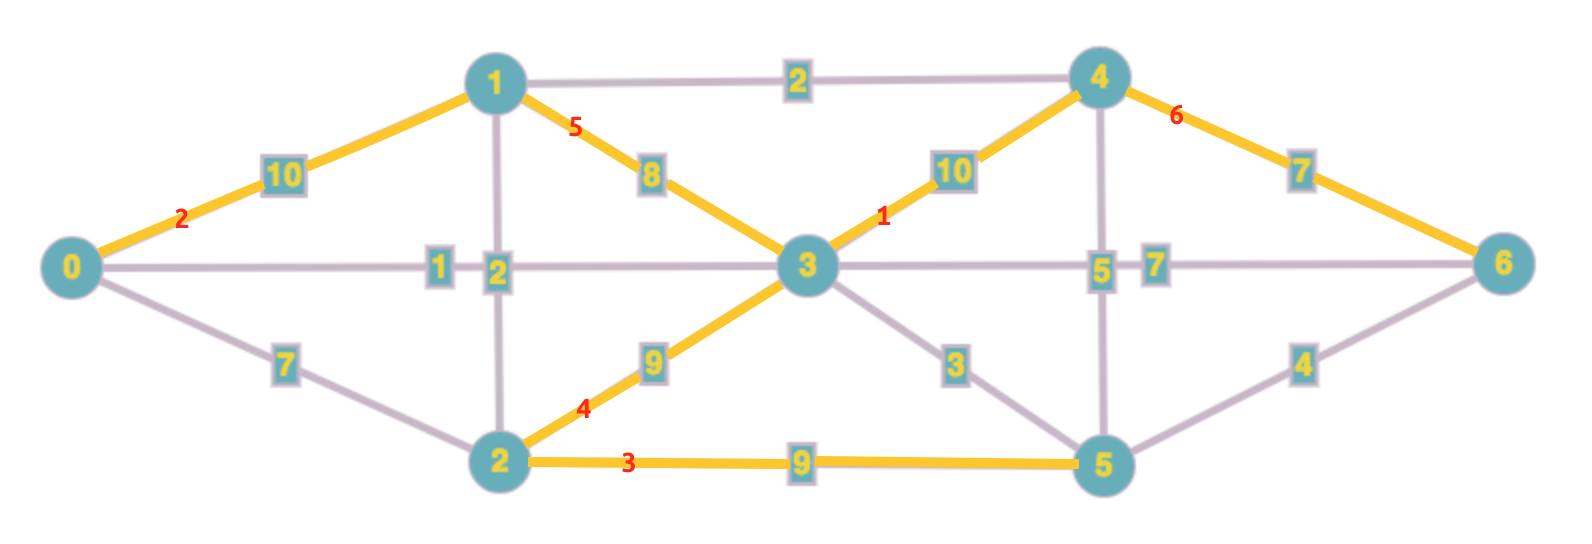
\includegraphics[width=0.8\textwidth]{graph3.png}
    \caption{Минимальный остов максимального веса}
\end{figure}

Вес остова: $W_{max} = 10+10+9+9+8+7=53$ \\

\end{document}